\section{theory}\label{theory}

\subsection{Abstract Domains}\label{subsec:abstract_domains}

In the following sections we will describe the abstract domains of our value analysis.

\subsubsection{Abstract domain of strings as regular expressions}\label{subsubsec:abstract_domains_strings}

To represent the abstract domain of the family SQL strings data types we have chosen regular expressions/languages.
Regular expressions/languages are chosen, as opposed to more powerful representations, for the decidable nature of inclusion and equality between them.

Let $REG$ denote the set of regular languages and
\begin{equation*}
    REG^{\leq n} = \{R \in REG \mid \forall w \in R : |w| \leq n\}.
\end{equation*}
In the following we do not distinguish between regular expressions and their languages.

In regards to abstract interpretation regulars expressions are not without their own quirks, as expressed in the following theorem.

The lattice of regular expressions $(REG, \subseteq, \cup, \cap)$ is not suited for abstract interpretation, as expressed by \autoref{thm:reg-lattice}.

\begin{restatable}{theorem}{reglattice}\label{thm:reg-lattice}
    $(REG, \subseteq, \cup, \cap)$ is a lattice, but not a complete one.
\end{restatable}

Thus we can not employ the Kleene fixed-point theorem to guarantee a fixed point and termination of our analysis.
We propose two solutions to overcome this limitation:
\begin{itemize}
    \item Limiting the size of the regulars expressions under consideration, this is sound in the case where the string data type which is abstracted over is fixed size;
    \item And to let the user define an abstract domain over the regular expressions that only contain finite elements.
\end{itemize}

To formalize the latter idea we introduce regular language partitions.

\begin{definition}
    Given a finite subset $REG^\subset \subset REG$ where $\bigcup REG^\subset = \Sigma^\star$.
    % todo Casper says: I am not sure if this restriction is useful.
    % and $\forall R_1, R_2 \in REG^\subset : R_1 \not\subset R_2 \land R_2 \not\subset R_1$.
    A regular language partition $p(REG^\subset)$ is a set where:
    \begin{itemize}
        % \item $\emptyset \in p(REG^\subset)$,
        \item $\forall R \in REG^\subset : R \in p(REG^\subset)$,
        \item $\forall R_1, R_2 \in p(REG^\subset) : R_1 \cup R_2 \in p(REG^\subset)$,
        \item $\forall R_1, R_2 \in p(REG^\subset) : R_1 \cap R_2 \in p(REG^\subset)$.
    \end{itemize}
\end{definition}

% Tikzfigures
\begin{figure}
    \resizebox{7.5cm}{!}{
        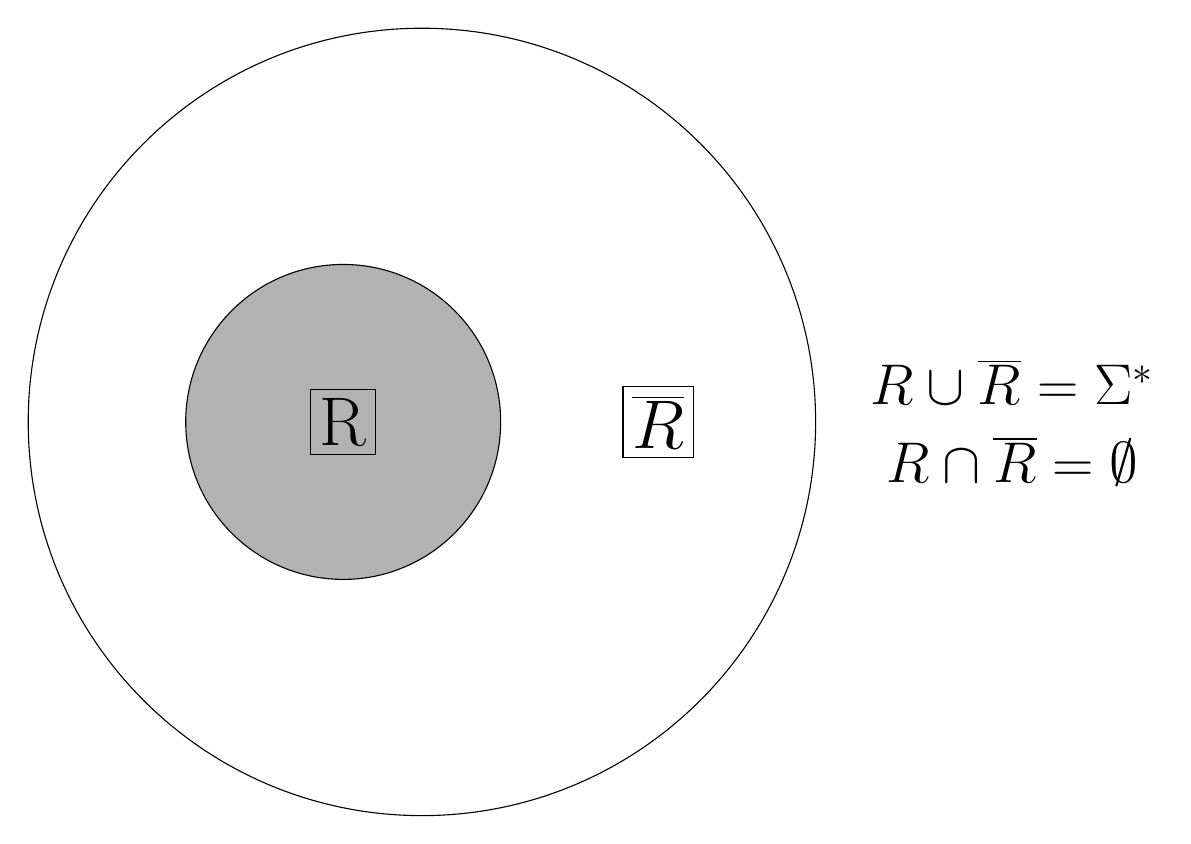
\begin{tikzpicture}
            \filldraw[fill=white, draw=black] (2,2) circle (5cm);
            \node [draw] at (5,2) {\Huge$\overline{R}$};
            \filldraw[fill=gray!60, draw=black] (1,2) circle (2cm);
            \node [draw] at (1,2) {\Huge R};
            \node at (9.5, 2.5) {\huge $R \cup \overline{R} = \Sigma^*$};
            \node at (9.5, 1.5) {\huge $R \cap \overline{R} = \emptyset$};
        \end{tikzpicture}
    }
    \caption{Regular language partition}
    \label{fig:tikz-reg-partition}
\end{figure}

\begin{figure}[!htb]
    \resizebox{6.5cm}{!}{
        \begin{tikzpicture}[scale = 0.5]
            \usetikzlibrary{calc}
            \node (a) [state] {\Huge$R \cup \overline{R} = \top = \Sigma^*$};
            \node (b1) [state, shift={($(a.south)+(3cm, -2.5cm)$)}] {\Huge $R$};
            \node (b2) [state, shift={($(a.south)+(-3cm, -2.5cm)$)}]{\Huge $\overline{R}$};
            \node (c) [state, shift= {($(a.south) + (0cm, -5.5cm)$)}] {\Huge $R \cap \overline{R} = \bot = \emptyset$};
            \draw (a) to (b1);
            \draw (a) to (b2);
            \draw (b1) to (c);
            \draw (b2) to (c);
        \end{tikzpicture}
    }
    \caption{Regular language partition as a lattice}
    \label{fig:tikz-reg-partition-lattice}
\end{figure}

\begin{theorem}\label{thm:finite-reg-lattice}
    $(REG^{\leq n}, \subseteq, \cup, \cap)$ is a complete lattice.
\end{theorem}

\begin{theorem}\label{thm:reg-partition-lattice}
    $(p(REG^\subset), \subseteq, \cup, \cap)$ is a complete lattice.
\end{theorem}


\subsubsection{Abstract domain of numbers as linear inequalities}\label{subsubsec:abstract_domains_numbers}


